\section{Patientsikkerhed}
Ved brug af medicinsk udstyr er sikkerheden for patienten vigtig, da patienter ofte er hæmmet eller svækket, og derfor er yderligere følsom. Patientsikkerhed indebærer fokus på de fysiologiske konsekvenser patienten kan blive udsat for, når patienten bliver koblet til elektroniske kredsløb. Hvis ikke patienten sikkerhed er i orden, vil patienten opleve at blive en del at det elektroniske kredsløb, hvilket kan medføre alvorlige følger, da patienten vil blive udsat for elektrisk strøm. Når elektrisk strøm løber igennem biologisk væv, kan tre fænomener forekomme. De tre fænomener er: Modstandsopvarmning af væv, elektrokemiske forbrændinger og elektrisk stimulering af muskel- og nervevæv. [1] 
\begin{figure}[H]
	\centering
	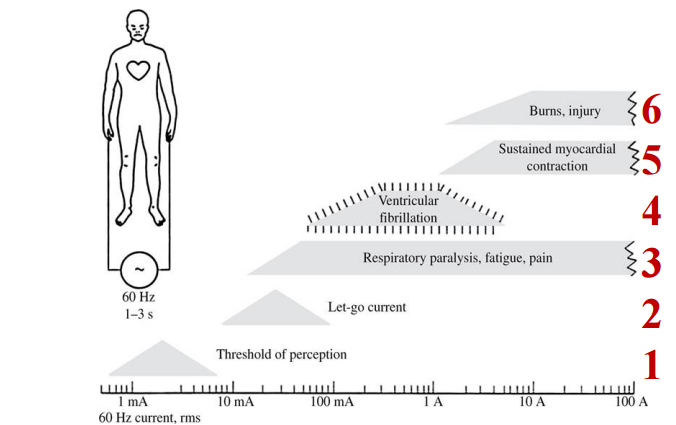
\includegraphics[scale=0.8]{figures/bProblemanalyse/Patientsikkerhed.png}
	\caption{Figuren viser den effekt størmmen har på patienten ved forskellige strømstyrker, og er inddelt i 6 stadier. Figuren er forudsat at personen har en vægt på 70 kg og at personen er i kontakt med et elektroninsk kredsløbet i 1-3 sekunder ved 60 Hz med begge hænder.}}
	\label{Patientsikkerhed}
\end{figure}

Figuren XX viser den effekt elektrisk strøm kan have på patienten ved forskellige strømstyrker. Ved den laveste strømstyrke, som er stadie 1, er strømmen mellem 0,5 mA og 10 mA. Ved stadie 1 vil patienten føle en prikkende fornemmelse og strømtætheden er stor nok til at aktivere nervesensorerne i huden, hvilket kan give en let opvarmning af huden. Ved stadie 2 udsættes patienten for en elektrisk strøm mellem 10 mA og 100 mA. Dette er den maksimale strøm, hvor patienten kan afbryde kontakten med strømmen frivilligt. Patienten vil opleve en kraftig påvirkning af muskler og nerver, hvilket resulterer i muskeltræthed og smerte, da musklerne skal lave ufrivillige kontraktioner. I stadie 3 er strømstyrken mellem 20 mA og 100 A og her kan patienten opleve åndedrætslammelser, smerter og muskeltræthed. Dette kan desuden resulterer i kvælning, hvis strømmen ikke afbrydes. Ved stadie 4, som ligger mellem 75 mA og 4 A, kan patienten opleve ufrivillig kontrahering af hjertemuskulaturen, hvilket kan medføre ventrikelflimmer. I det 5. stadie er der en strømstyrke på mellem 1 A og 100 A, og har sker der kontraktioner af den samlede hjertemuskulatur, hvilket kan resulterer i hjertestop, da, da hjertet er konstant kontraheret og derfor ikke kan videregive elektriske signaler. Ved det 6. og sidste stadie vil patienten opleve stærk strøm, som kan medføre alvorlige brandsår på huden, og ved store strømstyrker kan muskelkontraktioner blive så kraftige, at musklen og knoglerne kan løsrive sig fra hinanden. Derudover vil hjernen og nervevæv miste alle funktioner, når så store strømme løber gennem kroppen. Som det ses på figur XX kan flere af stadierne overlappe hinanden og foregå samtidig. [1]

Der er forskel på hvordan den elektriske strøm løber igennem kroppen, hvilket kan være medvirkende til hvor skadende strømmen er på patienten. De to forskellige måder kaldes makro- og mikrochok. Makrochok er når strømmen løber igennem kroppen ved to punkter på hudens overflade, og derved går kun en mindre del af strømmen igennem hjertet. Mikrochok er til gengæld, hvor det meste af strømmen løber igennem hjertet, da strømmen kommer fra et punkt på hudens overflade og forekommer hos patienter med elektriske ledere i hjertet f.eks. katetere. [1]

Så det er vigtigt at have fokus på patientsikkerhed når, der skal fremstilles medicinsk udstyr, som skal tilsluttes patienter. Dette kan gøre med jordforbindelse i systemet, eller ved at sørge for der ikke er direkte kontakt mellem patienten og elnettet, da store mængder strøm kan have alvorlige konsekvenser for patientens heldbred. 


[1] - Medical Instrumentation: Application and Design. Webster, John G. 2009.